\documentclass[11pt]{article}
\usepackage[margin=1in]{geometry}
\usepackage{amsmath}
\usepackage{amssymb}
\usepackage{enumitem}
\usepackage{tikz}

\title{ECON 20100: Elements of Economic Analysis II\\Problem Set 2 - Ellis Garver}
\date{Due: Monday, February 2, 2026}
\author{}

\begin{document}

\maketitle

\noindent\textbf{Instructions:} Show all work. Answers without justification will receive partial credit at best. You may work in groups, but each student must submit their own write-up.

\vspace{0em}
\noindent\rule{\textwidth}{0.4pt}

\section*{Question 1: Profit Maximization (25 points)}

A competitive firm has the cost function:
\[
C(y) = 50 + 2y + \frac{y^2}{2}
\]
The market price is $P = 12$.

\begin{enumerate}[label=(\alph*)]
    \item (3 pts) What are the firm's fixed costs and variable costs?
    \item[] Fixed costs: 50, Variable costs: $2y+\frac{y^2}{2}$
    
    \item (5 pts) Derive the firm's marginal cost function $MC(y)$.
    \item[] $MC(y)=\frac{\partial C(y)}{\partial y}=2+y$
    
    \item (5 pts) Find the profit-maximizing output $y^*$ using the condition $P = MC$.
    \item[] $P=MC\Rightarrow12=2+y\Rightarrow y^*=10$
    
    \item (5 pts) Calculate the firm's profit at $y^*$. Is the firm making positive, zero, or negative economic profit?
    \item[] Profit: $P\cdot y^*-C(y^*)=12\cdot 10-(50+2(10)+\frac{10^2}{2})=120-50-20-50=0$
    \item[] The firm is making zero economic profit at $y^*$
    
    \item (4 pts) Derive the firm's average variable cost function $AVC(y)$. At what output is AVC minimized, and what is the minimum AVC?
    \item[] $AVC(y)=\frac{VC(y)}{y}=\frac{2y+y^2/2}{y}=2+\frac{y}{2}\Rightarrow\frac{\partial AVC(y)}{\partial y}=0\Rightarrow\frac{1}{2}\neq0$, 
    \item[] $AVC(y)$ is linear and increasing so $AVC(y)$ is minimized at the smallest output level ($y=0$)
    \item[] Minimum $AVC(y)=AVC(0)=2$
    
    \item (3 pts) Should this firm produce or shut down in the short run? Explain using the shutdown condition.
    \item[] Shutdown condition: a firm should shut down if $P<\text{minimum}\; AVC$. Fixed costs are fixed. If the price is lower than $AVC$ then revenue does not cover variable costs and producing increases losses, so the firm should shut down in the short run. In this case $P=12>2=AVC(0)$ (minimum), so the firm should continue to produce in the short run.
\end{enumerate}

\vspace{0em}
\noindent\rule{\textwidth}{0.4pt}

\section*{Question 2: The Supply Curve (20 points)}

Consider a firm with marginal cost $MC(y) = 4 + 2y$ and average variable cost $AVC(y) = 4 + y$.

\begin{enumerate}[label=(\alph*)]
    \item (4 pts) At what price does the firm shut down? Find the minimum of AVC.
    \item[] $\frac{\partial AVC(y)}{\partial y}=0\Rightarrow1\neq0$, minimum $AVC(y=0)=4$
    \item[] The firm shuts down when $P<4$
    
    \item (6 pts) For prices above the shutdown point, derive the firm's supply function $y(P)$ by inverting the $P = MC$ condition.
    \item[] $P=MC(y)=4+2y\Rightarrow 2y=P-4\Rightarrow y(P)=\frac{P-4}{2}$
    
    \item (4 pts) Write down the complete short-run supply function, including the shutdown region.
    \item[] $y(P)= \begin{cases}
        0,\; P<4 \\ \frac{P-4}{2},\; P\geq 4
    \end{cases}$
    
    \item (6 pts) If there are 50 identical firms in this market, derive the market supply function $Y(P)$.
    \item[] $Y(P)=50\cdot y(P)\Rightarrow\begin{cases}
        50\cdot 0,\; P<4\\ \frac{50}{2}(P-4),\; P\geq 4
    \end{cases}\Rightarrow Y(P)=\begin{cases}
        0,\; P<4\\ 25(P-4),\; P\geq 4
    \end{cases}$
\end{enumerate}

\vspace{0em}
\noindent\rule{\textwidth}{0.4pt}

\section*{Question 3: Short-Run and Long-Run Equilibrium (25 points)}

Consider a competitive market with demand $Q_D = 1000 - 20P$ and 40 identical firms, each with cost function:
\[
C(y) = 10 + 2y + y^2
\]
(You can verify: $MC(y) = 2 + 2y$, $AVC(y) = 2 + y$, $ATC(y) = \frac{10}{y} + 2 + y$.)

\begin{enumerate}[label=(\alph*)]
    \item (4 pts) Derive the individual firm's supply curve (for $P$ above shutdown).
    \item[] $P=MC(y)=2+2y\Rightarrow 2y=P-2\Rightarrow y(P)=\frac{P-2}{2}$
    
    \item (4 pts) Derive the market supply curve with 40 firms.
    \item[] $Y(P)=40\cdot y(P)=\frac{40}{2}(P-2)=20(P-2)$
    
    \item (5 pts) Find the short-run equilibrium price $P^*$ and market quantity $Q^*$.
    \item[] $Q_D=Y(P)\Rightarrow 1000-20P=20(P-2)\Rightarrow1000-20P=20P-40\Rightarrow1040=40P\Rightarrow P^*=26$
    \item[] $Q_D(P^*=26)=1000-20(26)\Rightarrow Q^*=480$
    
    \item (4 pts) At this price, how much does each firm produce? What is each firm's profit?
    \item[] $y(P^*=26)=\frac{26-2}{2}=12$
    \item[] Profit: $P^*\cdot y(P^*=26)-C(y)=26\cdot12-(10+2(12)+12^2)=312-10-24-144=134$
    
    \item (4 pts) Based on your answer to (d), will firms enter or exit in the long run? Explain.
    \item[] Since profit $>0$, firms will enter in the long run.  Positive profits signal that firms are making economic profits (ie. resources earn more in this industry than their opportunity cost), so new firms enter to get a share of the profit. As firms enter, market supply increases, pushing prices down, and shrinking profits until $P=ATC$ and economic profits $=0$. 
    
    \item (4 pts) Find the long-run equilibrium price. (Hint: In long-run equilibrium with free entry, $P = ATC_{\min}$. Find where ATC is minimized.)
    \item[] $\frac{\partial ATC(y)}{\partial y}=0\Rightarrow\frac{-10}{y^2}+1=0\Rightarrow1=\frac{10}{y^2}\Rightarrow y^2=10\Rightarrow y=\sqrt{10}$
    \item[] $\frac{\partial^2ATC(y)}{\partial y^2}=\frac{20}{y^3}\Rightarrow\frac{\partial^2ATC(y=\sqrt{10})}{\partial y^2}=\frac{20}{(10)^{3/2}}>0$, so indeed a minimum
    \item[] $P=ATC_{\text{min}}=\frac{10}{\sqrt{10}}+2+\sqrt{10}\Rightarrow P_{\text{LR}}=2+2\sqrt{10}$
\end{enumerate}

\vspace{0em}
\noindent\rule{\textwidth}{0.4pt}

\section*{Question 4: The Edgeworth Box (20 points)}

Consider a pure exchange economy with two consumers (A and B) and two goods (X and Y). The total endowment is 10 units of X and 8 units of Y. Consumer A has the endowment $\omega^A = (7, 2)$ and consumer B has $\omega^B = (3, 6)$.

Their utility functions are:
\[
U^A(x, y) = xy \qquad U^B(x, y) = xy
\]
(Note: Both consumers have identical Cobb-Douglas preferences.)

\begin{enumerate}[label=(\alph*)]
    \item (4 pts) Verify that the endowments sum to the total. Draw an Edgeworth box with the appropriate dimensions and mark the initial endowment point $\omega$.
    \item[] $3+7=10=X,\; 6+2=8=Y$
    \item[] $\omega=(7,2)$ from origin/Consumer A perspective and $\omega=(3,6)$ from Consumer B perspective
    \item[] Utility functions downward sloping, strictly convex, asymptotic to the axes
    \begin{center}
    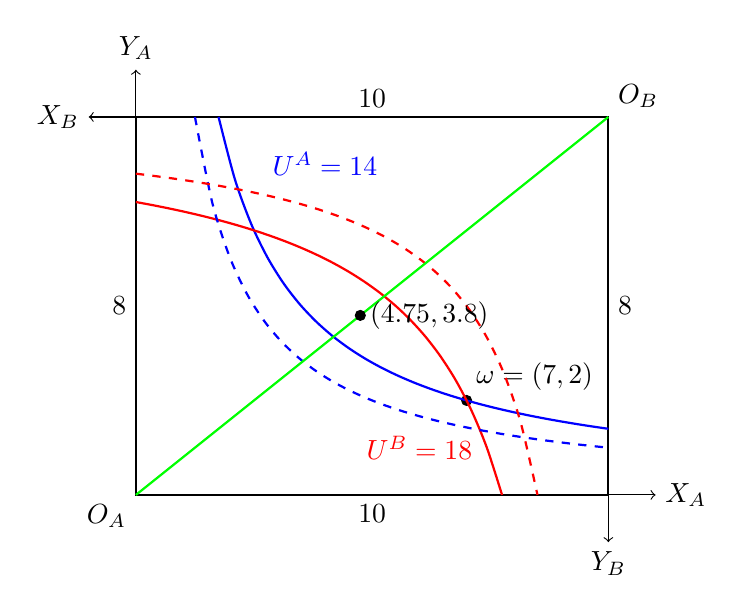
\begin{tikzpicture}[scale=0.6]
    
    % Edgeworth box (total endowment)
    \draw[thick] (0,0) rectangle (10,8);
    
    % Origins
    \node[below left] at (0,0) {$O_A$};
    \node[above right] at (10,8) {$O_B$};
    
    % Axes for A
    \draw[->] (0,0) -- (11,0) node[right] {$X_A$};
    \draw[->] (0,0) -- (0,9) node[above] {$Y_A$};
    
    % Axes for B
    \draw[->] (10,8) -- (-1,8) node[left] {$X_B$};
    \draw[->] (10,8) -- (10,-1) node[below] {$Y_B$};

    \node[below] at (5,0) {$10$};
    \node[left] at (0,4) {$8$};
    \node[above] at (5,8) {$10$};
    \node[right] at (10,4) {$8$};
    
    % Initial endowment
    \filldraw (7,2) circle (3pt);
    \node[above right] at (7,2) {$\omega = (7,2)$};

    % A's indifference curve passing through endowment
    \draw[domain=1.75:10, smooth, variable=\x, blue, thick]
      plot ({\x},{14/\x});
    
    % B's indifference curve passing through endowment
    \draw[domain=0:7.75, smooth, variable=\x, red, thick]
      plot ({\x},{8 - 18/(10-\x)});
    
    % Optional: additional curves inside box
    \draw[domain=1.25:10, smooth, variable=\x, blue, thick, dashed]
      plot ({\x},{10/\x});
    \draw[domain=0:8.5, smooth, variable=\x, red, thick, dashed]
      plot ({\x},{8 - 12/(10-\x)});
    
    % Labels
    \node[blue] at (4,7) {$U^A=14$};
    \node[red] at (6,1) {$U^B=18$};

    \draw[domain=0:10, smooth, variable=\x, green, thick]
      plot ({\x},{0.8*\x});
    \filldraw (4.75,3.8) circle (3pt);
    \node[right] at (4.75,3.8) {$(4.75,3.8)$};
    
    
    \end{tikzpicture}
    \end{center}
    
    \item (5 pts) Compute $MRS^A$ and $MRS^B$ at the initial endowment. Is the initial allocation Pareto efficient? If not, describe qualitatively what trades would make both consumers better off.
    \item[] $MRS=\frac{MUx}{MU_y}=\frac{y}{x}$ for both A and B $\Rightarrow MRS^A=\frac{2}{7},\; MRS^B=\frac{6}{3}=2$
    \item[] Since $MRS^A\neq MRS^B$ the initial allocation is not Pareto efficient. Consumer A trading $X$ for $Y$ and Consumer B trading $Y$ for $X$ makes both consumers better off and levels their respective $MRS$ equal to one another (where $MRS^A=MRS^B=\frac{4}{5}$).
    
    \item (5 pts) Find the equation for the contract curve. (Hint: Set $MRS^A = MRS^B$ and use the feasibility constraints $x^A + x^B = 10$ and $y^A + y^B = 8$.)
    \item[] $MRS^A=MRS^B\Rightarrow\frac{y^A}{x^A}=\frac{y^B}{x^B}\Rightarrow x^B=10-x^A,\; y^B=8-y^A\Rightarrow\frac{y^A}{x^A}=\frac{8-y^A}{10-x^A}$, solve:
    \item[] $\Rightarrow y^A(10-x^A)=x^A(8-y^A)\Rightarrow y^A(10-x^A)=8x^A-x^Ay^A$
    \item[] $\Rightarrow y^A(10-x^A)+x^Ay^A=8x^A\Rightarrow y^A((10-x^A)+x^A)=8x^A\Rightarrow y^A(10)=8x^A$
    \item[] $\Rightarrow y^A=\frac{8}{4}x^A\Rightarrow y^A=\frac{4}{5}x^A$ (contract curve equation)
    
    \item (6 pts) At a competitive equilibrium, we know $MRS^A = MRS^B = p_X/p_Y$. Using your answer from part (c), find the equilibrium price ratio. Then, using the fact that A's budget constraint is $p_X x^A + p_Y y^A = p_X(7) + p_Y(2)$ and that at the optimum $MRS^A = p_X/p_Y$, solve for the equilibrium allocation $(x^A, y^A)$. Verify it lies on the contract curve.
    
    Hint: From $MRS^A = y^A/x^A = p_X/p_Y$, you can express $y^A$ in terms of $x^A$ and the price ratio, then substitute into the budget constraint.
    \item[] At equillibrium: $\frac{p_x}{p_y}=\frac{y^A}{x^A}=\frac{4}{5}$
    \item[] Substitute $y^A=\frac{4}{5}x^A$ into A's budget constraint: $p_xx^A+p_y(\frac{4}{5}x^A)=p_x(7)+p_y(2)$
    \item[] $\Rightarrow p_xx^A-p_x(7)=p_y(2)-p_y(\frac{4}{5}x^A)\Rightarrow p_x(x^A-7)=p_y(2-\frac{4}{5}x^A)\Rightarrow \frac{p_x}{p_y}=\frac{4}{5}=\frac{2-\frac{4}{5}x^A}{x^A-7}\Rightarrow 4(x^A-7)=5(2-\frac{4}{5}x^A)\Rightarrow 4x^A-28=10-4x^A\Rightarrow8x^A=38\Rightarrow x^A=\frac{38}{8}=\frac{19}{4}=4.75$
    \item[] $\Rightarrow y^A=\frac{4}{5}(\frac{19}{4})=\frac{19}{5}=3.8$, so $(x^A,y^A)=(4.75,3.8)$, lies on contract curve
\end{enumerate}

\vspace{0em}
\noindent\rule{\textwidth}{0.4pt}

\section*{Question 5: Conceptual Questions (10 points)}

Answer each of the following briefly but precisely.

\begin{enumerate}[label=(\alph*)]
    \item (3 pts) A firm is currently producing where $P = 15$ and $MC = 10$. What should the firm do, and why?
    \item[] Since $P>MC$, the firm should increase output to raise profit because at this level producing more increases revenue faster than the subsequent costs.
    
    \item (3 pts) In the short run, a firm has $P = 8$, $AVC = 6$, and $ATC = 12$. Should the firm produce or shut down? Is it making a profit or loss?
    \item[] Since $P>AVC$, the firm should produce in the short run because revenue will cover the variable costs which minimizes losses due to $P<ATC$.
    
    \item (4 pts) Explain in words why, in a competitive equilibrium of an exchange economy, the allocation must be Pareto efficient. Your answer should reference the relationship between MRS and prices.
    \item[] In competitive equilibrium for an exchange economy, each individual maximizes utility given prices so $MRS=\frac{p_x}{p_y}$. Since each individual faces the same price ratio, no mutually beneficial trade remains, the equilibrium allocation lies on the contract curve, and is Pareto efficient. 
\end{enumerate}

\vspace{0em}
\noindent\rule{\textwidth}{0.4pt}

\vspace{1em}
\noindent\textbf{Total: 100 points}

\end{document}